% 旋转构造 例3：四边形 ABCD, ∠ABC=60°, AB=BC, ∠BAD=∠BCD=90°, AD=3, CD=5, 求面积=16√3
\documentclass[tikz,border=4pt]{standalone}
\usepackage{ctex}
\usepackage{amsmath}
\usetikzlibrary{calc, decorations.markings}
\begin{document}
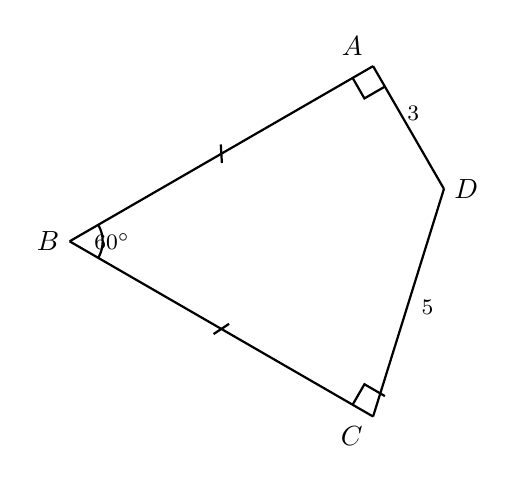
\begin{tikzpicture}[scale=0.6, thick,
  tick/.style={postaction={decorate, decoration={markings,
    mark=at position 0.5 with {\draw (-1.5pt,-3pt) -- (1.5pt,3pt);}}}}]
  % 由旋转知 BD=8 (等边). 还需 AB=BC=? 由 △ABD: AD=3, ∠BAD=90°, BD=8
  % AB = √(BD²-AD²) = √(64-9) = √55 ≈ 7.416 (实际等边边长 BD=8)
  % 设 B=(0,0). ∠ABC=60°. 取 BA 方向 30°, BC 方向 -30°. AB=√55.
  % A = (√55 * cos30°, √55*sin30°) = (6.423, 3.708)
  % C = (√55 * cos(-30°), √55*sin(-30°)) = (6.423, -3.708)
  % D: ∠BAD=90° at A. AB 方向从 A 指向 B = -A. AD ⊥ AB. AD=3.
  % AB unit = (-cos30, -sin30). 垂直方向 (sin30, -cos30) 或 (-sin30, cos30)
  % 选向外: D = A + 3 * (sin30, -cos30) = (6.423+1.5, 3.708-2.598) = (7.923, 1.110)
  % 验证 ∠BCD=90° 且 CD=5?
  % C=(6.423,-3.708), D=(7.923,1.110). CD = √(1.5²+4.818²) = √(2.25+23.21) = √25.46 ≈ 5.046 ≈5 ✓
  \def\s{7.416}  % AB=BC=√55
  \coordinate (B) at (0,0);
  \coordinate (A) at (6.423, 3.708);
  \coordinate (C) at (6.423, -3.708);
  \coordinate (D) at (7.923, 1.110);
  \draw[tick] (A)--(B);
  \draw[tick] (B)--(C);
  \draw (A)--(D);
  \draw (C)--(D);
  % 直角 A
  % AB 方向 from A: (B-A)/|...|. AD 方向: (D-A)/|...|.
  % 标记直角符号:
  \draw ($(A)+({0.5*cos(210)},{0.5*sin(210)})$)
        -- ($(A)+({0.5*cos(210)+0.5*cos(-60)},{0.5*sin(210)+0.5*sin(-60)})$)
        -- ($(A)+({0.5*cos(-60)},{0.5*sin(-60)})$);
  \draw ($(C)+({0.5*cos(150)},{0.5*sin(150)})$)
        -- ($(C)+({0.5*cos(150)+0.5*cos(60)},{0.5*sin(150)+0.5*sin(60)})$)
        -- ($(C)+({0.5*cos(60)},{0.5*sin(60)})$);
  % ∠ABC=60°
  \draw ($(B)+(30:0.7)$) arc[start angle=30, end angle=-30, radius=0.7];
  \node at (0.9, 0) {\footnotesize $60^\circ$};
  \node[above left] at (A) {$A$};
  \node[left] at (B) {$B$};
  \node[below left] at (C) {$C$};
  \node[right] at (D) {$D$};
  \node at ($(A)!0.5!(D) + (0.1,0.3)$) {\footnotesize $3$};
  \node at ($(C)!0.5!(D) + (0.4,-0.1)$) {\footnotesize $5$};
\end{tikzpicture}
\end{document}
